\documentclass[12pt,letterpaper]{article}

\usepackage{ifpdf}
\usepackage{mla}
\usepackage{graphicx}


\begin{document}
\begin{mla}{Cameron}{Carroll}{Prof. Mood}{English 124}{\today}{Paradigm Shift: Awareness is Key}

While we all coexist tangibly in the existing world, each of us has our own private existence where things happen just the way we expect them to. Usually, people have the ability to cull this inner paradigm, staying focused and quite aware of the outside world. As our focus slips, however, things tend to slip back into our automatic world; Our brains, as pattern machines, recognize when a value matches what we seek. They may also ignore the true value and simply project what they are seeking instead, causing a person to see or hear something that did not happen. Some of us have excellent presence of mind and willpower, enabling them to be far more astute than others. On the other end of the scale, some people are completely bound by their own interpretation of the world, and cannot escape. This is our paradigm, our worldview; It is the set of intellectual dispositions, cultural histories and personal experiences, all rolled into one way of looking at the world. Everything a person has ever thought or done contributes to the worldview, and understanding this is to understand oneself more deeply than many ever venture.

As the Center Leo Apostel, a Belgian research department focusing on complexity and world dynamics, puts it, ``A world view is a coherent collection of concepts and theorems that must allow us to construct a global image of the world, and in this way understand as many elements of our experience as possible.'' [CLeA] In this definition, the distinction is made that worldview is a tool for understanding the world. We don't know everything about our environment, so we fill in the blank spaces using prediction. This prediction is subconscious, automatic and its power is so inconspicuous that almost all people judge and weigh using it every day. 

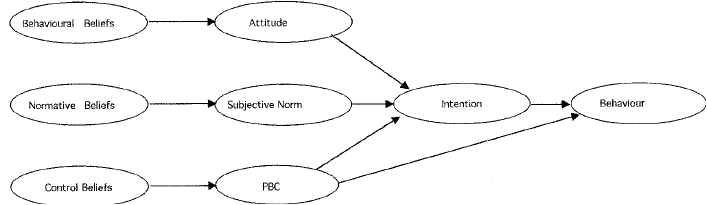
\includegraphics{fig1.png}
{\small Figure 1 taken from Armitage \& Conner. The theory of planned behavior is shown, with PBC being perceived behavioral control, or a person's own confidence in their ability to perform a behavior.}
\vspace{7 mm}

As shown in figure 1, a number of factors contribute to intention and behavior, and all of them stem from worldview.  
``Subjective norm refers to the individual's perceptions of general social pressure to perform (or not to perform) the behavior.'' … ``Attitude towards the behavior reflects the individual's global positive or negative evaluations of performing a particular behavior.'' [Armitage \& Conner 4] Of these two variables, the former is concerned with community aspects of worldview, and the latter is concerned with oneself. A person synthesizes an expected outcome for their actions based on previous event / consequence pairs. Simply put, their worldview dictates what they expect will happen, and therefore dictates whether or not a person will perform that action.

A surreal feeling occurs when one rises too quickly: Blood rushes to the head and, depending on physiology and hydration, can range from light-headedness to losing consciousness. Waking from this brief unconscious state is strange because one finds that while gone, life went on: the body may have kept walking, or it ay have managed to stay standing. Maybe it fell down and lies sprawled on the floor, but a few seconds later the mind reawakens, reconnects and suddenly asks, “What the heck happened?”  The body and brain are machines that keep working, and keep thinking and keep making decisions even when your mind is turned off. A second example of this can be seen on the face of an enraged man as he calms; One can literally see the rage leave their eyes and a deep regret develops. His consciousness was not in control, instead yielding to the pattern and chemical overlords; We are slaves to our physiology.

Worldview is a highly personal matter, encompassing experience and attitude. My own is simple: Empirical, secular and analytical. I believe in no gods, deities, luck or coincidence. D\'{e}j\`{a}-vu, in my world, is best explained as a memory error in the brain rather than a creepy reoccurance of an event. I find the good in people is almost never selfless... there is motive behind every action. Contrary to this, I find that the bad in people is almost never evil, but greed or selfishness or thoughtlessness. I feel a stronger relationship to city and sprawl than nature: The beauty of forests and plains is equal to the beauty of engineering and endless lights. The sanctity of the human body, whether one finds it sacred for religious reasons or because it's a beautiful, complex machine, should be augmented and experimented with and pushed to the limits. These dispositions and feelings are part of my persistent day-to-day paradigm. But they are, ultimately, no more significant than those dispositions that I cannot immediately consider. Those are the thoughts and feelings that run so deep and so far back that I don't even know that they've happened, and that subconscious pattern machine inside is often in control more than I. 

We would all love to believe that we are self made and self defined. The American dream, fleeting as it may be, encompasses these values. That itself is, rather ironically, part of our cultural history and upbringing as Americans. My values of scientific trust and secular life I believe are sourced to my parents, who have said that they had originally intended to expose their children to all religions. Instead, we were raised according to their beliefs, which lack a spiritual realm. The natural alternative to spirituality is a scientific basis, which while not always logical certainly provides the most fair explanation. The tendency to be an apathetic technologist was relatively recent: A comfortable middle class life combined with being surrounded by technology and being encouraged to become heavily involved in its development and use are all factors that may contribute.

I may be a pessimistic, and occasionally closed-minded thinker: In terms of people suggesting ideas, I don't shut them down or disagree with them necessarily. I'm perfectly willing to accept and discuss the vast majority of issues.. but there are some social, economic and abstraction issues that really grind my gears. I find that when something like that is brought up, I immediately reject it without knowing or intending to: My previous experiences and future expectations make their suggestion seem so grim and so abhorrent that my mind won't accept it initially, even if it later seems perfectly reasonable. Awareness of these kinds of issues, I feel, is a very simple and very easy way to stop yourself from being controlled by your deep emotions and dispositions. 

 As aforementioned, malice stems from ignorance and ignorance is, truly, the opiate of the masses. By not realizing that they have a worldview to explore, most members of our society are not independent thinkers: To ride the ebb and tide of rhetoric is the ultimate insult to one's intellect. Intellectual dispositions and an articulated worldview are the first steps to understanding oneself and one's own decision-making process. We are not doing our duty as good citizens of the world if we are content to lie in the dark; Every one of us should strive to see more than the shadows on the wall.

\begin{workscited}

\bibent
Armitage, Christopher. \& Conner, Mark. ``Efficacy of the Theory of Planned Behavior: A meta-analytic review." \textit{British Journal of Social Psychology}, 2001

\bibent
Aerts, D; Apostel, L; DeMoor, B; Hellemans, S; Maex, E; Van Belle, H; Van Der Veken, J; ``Worldviews: From Fragmentation to Integration" VUB Press, Brussels, 1994 

\end{workscited}


\end{mla}
\end{document}
